\chapter{}

\autoref{tpgmmtrain} show the training function for TPGMM training. This function handles all computation steps for training a TPGMM model. This code block is used to train the the TPGMM model. It is saved into a pickle file to allow offline computation and online application.

\lstinputlisting[language=Python, 
caption=TPGMM training function, label=tpgmmtrain]{code/gmm_train.py}

\autoref{gmrtrain} show the training function for GMR training. This function handles all computation steps for GMR. 

\lstinputlisting[language=Python, 
caption=GMR training function, label=gmrtrain]{code/gmr.py}

\autoref{intergration} shows the Python implementation for RK4 to forward integrate a RBDL model. This is can be generlized for any RBDL model with an arbitrary torque or force command. This is useful for simulating the model forward input to test the dynamics of a system or for the iLQR forward pass. This code can be translated into C++ for improve computational speeds. 

\lstinputlisting[language=Python, 
caption=This block shows how to integrate a RBDL model using Runge-Kutta 4, label=intergration]{code/intergration.py}

\autoref{riccati} show the Python code for the algebraic riccati equation along a predefined path. In this implementation the $Qs$ are a list matrixes that are the same length as the path. The computation is performed using backward integration from the goal to the start position.  

\lstinputlisting[language=Python, 
caption=Solving the algebraic riccati equation, label=riccati]{code/riccati.py}


The following block is used to program the Atlas motor drivers. It need to be flashed to the each of the controller using Pro-Motion \footnote{\href{https://www.pmdcorp.com/products/development-software}{https://www.pmdcorp.com/products/development-software}}. These script was tuned to the specific DC motors using on the system. It should also be noted that the scripts can be auto generated using the Axis wizard in the program, however this will put lines with "\# Axis 1" line the script. These lines need to be deleted before the script can be flashed to the driver. They will cause checksum error when flashing the driver.   

\begin{lstlisting}
'Lines preceded with ' are comments and are included here to reveal a command's enumerated parameter value.

SetMotorType 7
SetPWMFrequency 5000
SetCurrentControlMode 0
'SetFOC 512 0 
'SetFOC 513 0 
'SetFOC 514 16384 
SetCurrentLoop 512 1395 
SetCurrentLoop 513 1813 
SetCurrentLoop 514 16383 
' SetCurrentFoldback ContinuousCurrentLimit(0) 6486 
SetCurrentFoldback 0 6486 
' SetCurrentFoldback I2tEnergyLimit(1) 617 
SetCurrentFoldback 1 617 
' SetDriveFaultParameter OvervoltageLimit(0) 38207 
SetDriveFaultParameter 0 38207 
' SetDriveFaultParameter UndervoltageLimit(1) 7347 
SetDriveFaultParameter 1 7347 
' SetDrivePWM Limit(0) 16384 
SetDrivePWM 0 16384 
' SetDriveFaultParameter WatchdogLimit(3) 5 
SetDriveFaultParameter 3 0 
' SetDriveFaultParameter TemperatureLimit(4) 19200 
SetDriveFaultParameter 4 19200 
' SetDriveFaultParameter TemperatureHysteresis(5) 1280 
SetDriveFaultParameter 5 1280 
Update 
SetFaultOutMask 0x0861
'SetDriveFaultParameter RecoveryMode(2) 1 
SetDriveFaultParameter 2 1 
' clear all errors
ClearDriveFaultStatus
ResetEventStatus 0
' Without this line the driver will not output current/torque
SetOperatingMode 0x7

\end{lstlisting}

\chapter{}

\autoref{fig:PhyicalModelSimulink} shows the simulink diagram for controlling the test system. The main difference between this system and the prevuis system is that this diagram has a block to communicate over serial. The controller send a new torque message when a new sensor reading is read over the serial port.

 \begin{figure}[h]
     \centering
     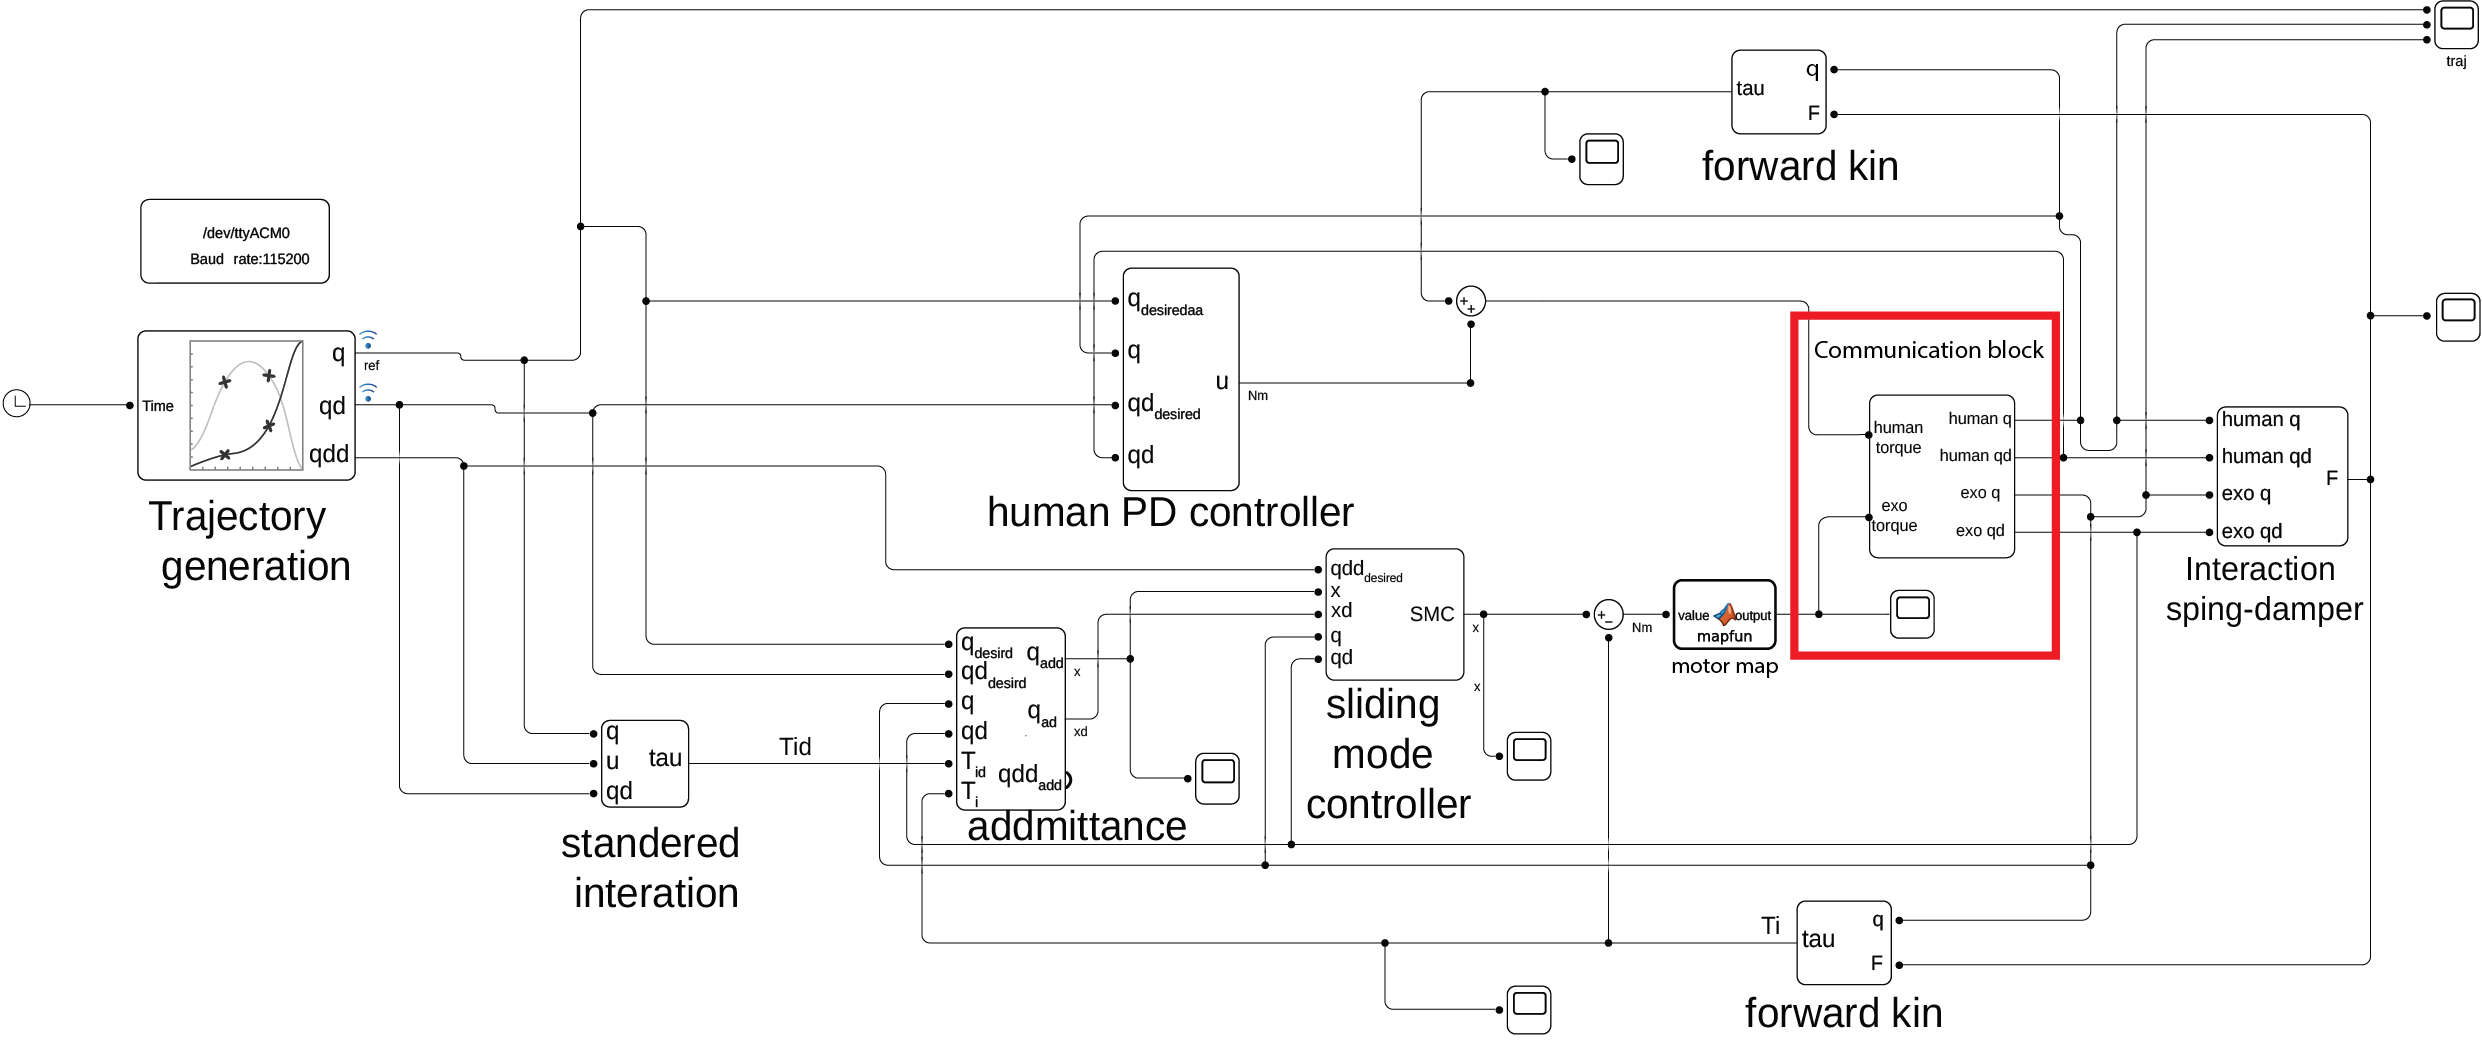
\includegraphics[width=\textwidth]{images/appendix/phyical_system_simulink.png}
     \caption[Simulink Controller]{Simulink Controller for physical test system, the communication is handled over a Serial port.}
     \label{fig:PhyicalModelSimulink}
\end{figure}


 \autoref{fig:admittanceSimulink} shows the implementation of the admittance controller with variable gains. 
 
\begin{figure}[h]
     \centering
     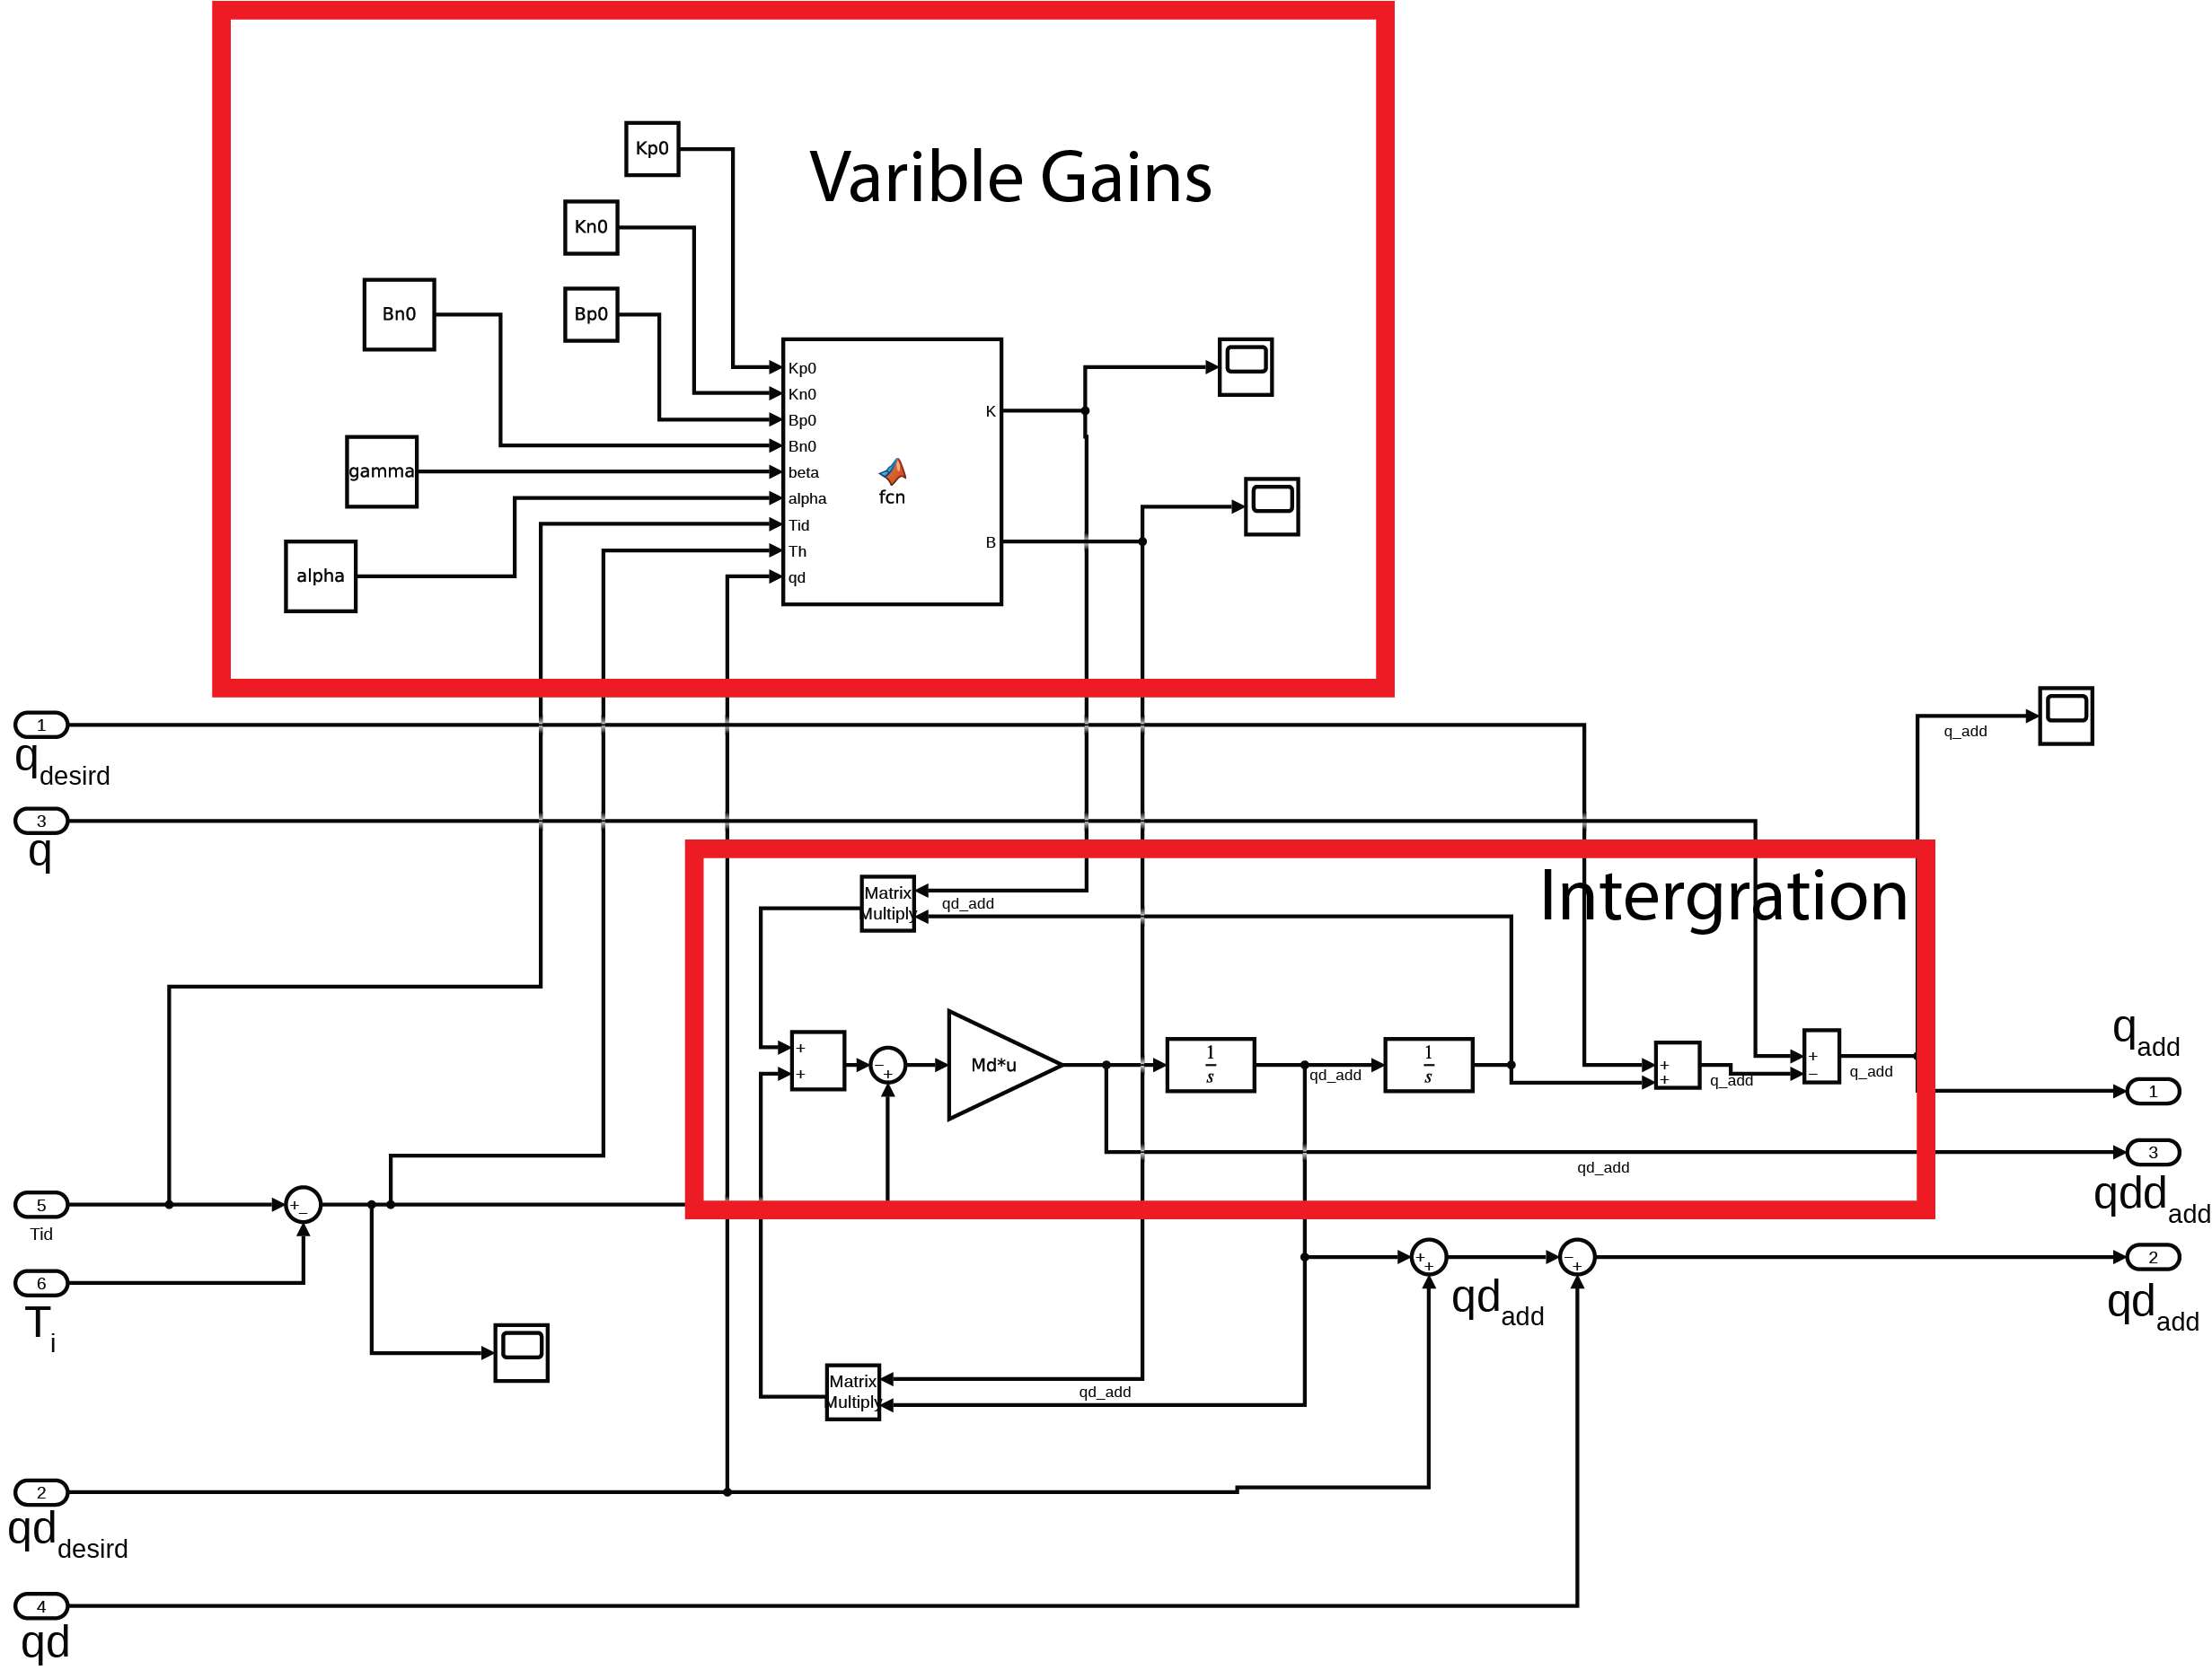
\includegraphics[width=\textwidth]{images/appendix/addmittance_simulink.png}
     \caption[Simulink Admittance Controller]{Admittance Controller with variable gains implementation in simulink.}
    \label{fig:admittanceSimulink}
\end{figure}







% iLQR code (maybe pshedo code)?? with link to real code

% \begin{algorithm}[t]
% \begin{algorithmic}[1]
% \Function{BackwardPass}{$X,U$}
% \State $p_N \;\leftarrow (l_N)_x + (c_N)_{x}^{T} (\lambda + I_{\mu,C_N})$
% \State $P_N \;\leftarrow (l_N)_{xx} + (c_N)_{x}^{T}I_{\mu,C_N}( C_{N}_x)$

% \State $(\hat{\boldsymbol \theta}, \hat{\bf r}) = \Call{Update}{{\boldsymbol \theta}, {\bf v}, {\bf r}, {\bf z}_u, \Sigma_u}$
% \State $(\hat\Lambda, \hat{\boldsymbol \eta}, A_u) = \Call{LinearSystem}{\hat{\boldsymbol \theta}\;, \hat{\bf r}}$

% \State $changedLP = \textsc{false}$
% \For{$it = 0$ \textbf{to} $it_{max}$}
%     \State $ {\boldsymbol \delta} = \Call{Solve}{\hat\Lambda, \hat{\boldsymbol \eta}} $
%     \If{$norm({\boldsymbol \delta}) < tol$}
%         \State ${\bf break}$
%     \EndIf
%     \State $\hat{\boldsymbol \theta}\;\leftarrow \hat{\boldsymbol \theta} \oplus {\boldsymbol \delta}$
%     \State $(\hat\Lambda, \hat{\boldsymbol \eta}) = \Call{LinearSystem}{\hat{\boldsymbol \theta}, \hat{\bf r}}$
%     \State $changedLP = \textsc{true}$ % we have just optimized, L needs to be rebuilt    
% \EndFor
% \Statex \Comment a simple incremental Gauss-Newton solver

% \State $ordering = \Call{AMD}{\hat\Lambda}$
% \State $\hat R = \Call{Chol}{\hat\Lambda, ordering}$ %%legit\Comment the $\hat R$ factor may be reused, if available in the solver

% \If{$changedLP$}
%     \State $\hat\Sigma = \Call{CalculateCovariance}{\hat R, ordering}$
% \Else
%     \State $\hat\Sigma = \Call{UpdateCov}{\Sigma, \hat R, ordering, A_u, {\bf v}}$ % UpdateCovariance was too long
% \EndIf
% \EndFunction
% \end{algorithmic}
% \caption{\label{alg:seeifrelin} BackwardPass}
% \end{algorithm}
